\documentclass[a4paper,10pt]{report}
\usepackage[utf8]{inputenc}
\usepackage[T1]{fontenc}
\usepackage{fancyhdr}
\usepackage[french]{babel}
\usepackage[authoryear, numbers]{natbib}
\usepackage[final]{pdfpages} 
\usepackage[unicode=true,hidelinks]{hyperref}
\usepackage[babel=true]{csquotes}
\usepackage{epigraph}
\usepackage{float}
\restylefloat{table}
\lhead[\rm\thepage]{\fancyplain{}{\sl{\rightmark}}}
\rhead[\fancyplain{}{\sl{\leftmark}}]{\rm\thepage}





\begin{document}
\title  {Titre du papier}
\author  {Thibault François }
\maketitle
%\lhead{\emph{Table des matières}}  % Set the left side page header to "Contents"
\tableofcontents  % Write out the Table of Contents

\chapter*{Introduction}

 
\chapter{Contexte} \label{contexte}




 
\chapter{Vers quelle gestion des compétences }
Maintenant que nous avons fait le tour du problème, il faut définir les objectifs à atteindre en s'aidant de la structure de l'organisation. Ensuite il faut définir quelle type de gestion des compétences sera la plus adapté pour atteindre les objectifs et finalement définir la méthodologie et un plan d'action pour sa mise en place. Mais avant toute chose, il faut s'accorder sur la définition de compétence. 

\section{Définition de la compétence}
Avant toutes choses, regardons ce qui se dit à propos de la notion de compétence dans la littérature. Commençons parce ce qu'il en est dit dans le livre de Guérin, Cadin, Pigeyre\citep[pp.170-171]{gestionressourceshumaine2007}
\begin{quotation}
\textit{ On observer une grande variété dans les définitions adoptées, mais toutes retiennent, d'une manière ou d'une autre les mêmes éléments essentiels:
\begin{itemize}
 \item La compétence prend sens para rapport à l'action: on ne peut parler de compétence que dans le cadre précis d'une situation de travail;
 \item Elle combine de façon dynamique les différents éléments qui la constituent (savoirs, savoir-faire pratiques, raisonnements) pour répondre à des exigences d'adaptation.
\end{itemize}}
\end{quotation}

Plus loin, on retrouve encore ce lien entre compétence et action.\citep[pp.172]{gestionressourceshumaine2007}
\begin{quotation}
 \textit{"La compétences est une notion abstraite et hypothétique."}\footnote{Leplat J., ``Compétence et ergonomie'', Modèle en analyse du travail, Bruxelles, Mardaga, 1991, pp. 263-278}
 \textit{On ne peut en observer que les manifestations. [...], c'est à partir de la situation de travail et de la manière dont celle-ci est assumée qu'il est possible d'inférer la compétence.}
\end{quotation}

Et finalement il ne faut pas oublier le caractère socialement construit de la compétence. \citep[pp.249]{gestionressourceshumaine2007}
\begin{quotation}
\textit{[...] c'est le fait de reconnaître une compétence qui la fait exister. Autrement dit, la compétence n'existe pas sans le jugement d'autrui: nul ne saurait se déclarer compétent lui-même.}
\end{quotation}

Nous pouvons observer un point de vue assez similaire dans Aubret, Gilbert\citep[pp.7]{evalcompetence} où la encore il ne s'accorde pas sur une définition de la compétence:

\begin{quotation}
\textit{La notion de compétence se présente souvent comme une notion insaisissable au regard de la diversité des usages. [...]
Le terme de compétence fait partie de ces mots à multiples facettes que personne n'a véritablement le pouvoir de réduire à une seule non équivoque et de l'imposer à tous.
Aussi, nous voyons apparaître dans la littérature sur les compétences de nombreuses définitions qui prennent ce mot, soir comme un terme, soit comme une notion, un concept ou un construit social. [...] R. Zemke (1995), [...], en arrive à la conclusion que la compétence, les compétences, les modèles de compétences et la formation axée sur la compétence sont des mots valises qui signifient seulement ce que l'auteur veut leur faire dire.}

\textit{Ce que disent les chercheurs et praticiens:}
\textit{\begin{itemize}
 \item Compétence: c'est la capacité à résoudre un problème dans un contexte donné (Michel \& Ledru, 1991);
 \item Les compétences sont des ensembles de connaissances, de capacités d'actions et de comportement structurés en fonction d'un but et dans une type de situations données (Gilbert \& Parlier, 1992);
 \item [...]
 \item La compétences est la prise d'initiative et de responsabilité de l'individu sur des situations professionnelles auxquelles il est confronté (Zarifian, 1999)
\end{itemize}}

\end{quotation}

Finalement l'article de Delobbe, Gilbert, Le Boudelaire\citep[pp.30]{delobbe} résume assez bien la complexité de la situation et résume les différentes approche dans le tableau \ref{def_comp}.
\begin{quotation}
\textit{Les définitions de la compétence ont été marquées par des divergences idéologiques qui se sont traduites dans la facon concrète de formuler les référentiels. Entre le savoir-faire opérationnel validé de l'accord ACAP 2000 et la compétence définie comme l'intelligence des situations par Bortef, entre les approches ergonomiques et sociologique francophones dans lesquelles la compétence est directement ancrée dans les activités des opérateurs et l'approche psychologique surtout nord-américaine, il y a des nuances importantes. }
\end{quotation}


\begin{table}
  \caption{Définitions et approches opérationnelles de la compétence\citep[pp.31]{delobbe}}
  \label{def_comp}

  \begin{center}
    \begin{tabular}{p{0.25\textwidth}|p{0.35\textwidth}|p{0.4\textwidth}}
       & \textbf{Contextualisation forte: compétences specifiques} & \textbf{Contextualisation faible: compétenes génériques}\\
       \hline
      \textbf{Prescription forte: contrôle externe des comportements}  & Savoir-faire élémentaires, gestes professionnels prédéfinis et prescrits (Accords ACAP 2000) & Normes de comportements et savoir-être partagés, traduisant l'adéquation aux valeurs plus ou moins explicite de l'entreprise (Schippman et al., 2000\\
      \hline
      \textbf{Prescription faible: autonomie accrue des travailleurs} & Savoir-agir complexes et autonomes en situation incertaine (Le Boterf, 1997; Zarifian, 2001)  & Connaissances, aptitudes, capacités et toutes caractéristiques psycologiques individuelles associées à un niveau élevé de performance (Boyatzis, 1982; McClelland, 1973; Spencer et Spencer, 1993)\\
    \end{tabular}
  \end{center}
\end{table}

\paragraph{}Il ressort que la compétence n'a pas de définition mais beaucoup s'accorde pour dire que la compétence ne peut s'exprimer que dans l'action. Sans action, il n'y a pas de compétence. La compétence est le plus souvent un mélange de savoir, savoir-faire et de capacité à raisoné. Pour construire notre méthode de gestion des compétences, il faudra donc tranché sur une défintion. Cette définition dépendra du contexte dans lequel nous voulons l'utiliser. Le tableau \ref{def_comp} lie celle-ci aux caractéristique de l'organisation qui va l'employer. C'est pour cela qu'avant de définir notre notion de compétence, nous allons nous atteler à définir la structure organisationelle d'Odoo.  

\section{Étude de la configuration organisationelle d'Odoo}
\subsection{La configuration en 2010}
Il est interressant de revenir à la configuration d'Odoo en 2010, juste après la première levée de fond. Comme on peut le voir dans le tableau \ref{nb_employe}, au début de l'année 2010 il y avait 18 employé et à la fin de l'année il y en avait déjà 34. Ce nombre reste faible comparé au 125 employés en belgique actuellement. A cette époque le sommet hierarchique était composé d'un CEO-fondateur\footnote{Chief Executive Officer}, CSO\footnote{Chief Sales Officer}, COO\footnote{Chief Operating Officer} et d'un CTO\footnote{Chief Technical Officer}. Il y avait déjà trois département, tous présent sur le même site. Le département de recherche et développement gérer par le CTO, le département de vente gérer par le CSO et le département de service en théorie gérer par le COO. En dehors du sommet hiérchique, il n'y avait pas de responsable d'équipe. Les employés sont depuis le début très qualifié: des ingénieurs en informatique en R\&D et au département de service et des ingénieurs des gestions au département de service et à la vente. Au sein de chaque département, le travail était intercheangable entre chaque membre d'un département. En R\&D et au PS\footnote{Abréviation pour les département de service: Professional Services}, chacun travaillait sur son projet et il est difficile de changer l'assignation en cours de route, mais toute nouvelle tâche était suceptible d'être assigné à quiconque. Le CEO passait presque quotidiennement voir qui faisait quoi pour donner quelque ajustement, débloquer une situation. Toutes les décisions était prise par le comité de direction composé des quatres membres exécutifs mais bien entendu le CEO avait toujours le dernier mots. C'est à cette époque le beau-frère de celui-ci fut envoyé pour ouvrir un bureau aux états-unis.  

\newpage
\paragraph{}Le tableau \ref{rh_2010} résume la situation au niveau des ressources humaines


\begin{table}[H]
  \caption{Résumé de la gestion des ressources humaines en 2010}
  \label{rh_2010}

  \begin{center}
    \begin{tabular}{l|p{0.85\textwidth}}
       Planification & Il nous manque des informtations pour pouvoir juger de la planification au niveau RH. Il semble que dans un contexte de croissance, le recrutement était ouvert pout les trois département.\\
       \hline
       Sélection & La sélection se faisait via une interview avec le directeur concerné ou alors directement avec le CEO. Dans un premier temps les interview était tout à fait informelle. Pour les postes techniques des exercices de programmation on été mis en place à la fin de 2010\\
       \hline
       Formation & Une semaine de formation était donné à tout les employés à leur arrivées. Une semaine supplémentaire est donné au profils techniques. Ces deux semaines de formation était dispensé car elle étaient vendues et prestées pour nos partenaires. Rien de spécifique à chaque poste n'existe. Pour cela il fallait se former sur le temps. Généralement, la méthode de formation consistait à jetté les nouveaux employés tout habillé dans la piscine.  \\
       \hline
       Evaluation & La notion d'évaluation n'était pas du tout formaliser, elle se faisait à le demande de l'employé principalement. A cette époque les seules personnent qui furent congédiée appartenaient au département de vente lorsque ceux-ci avaient de mauvais chiffres. En générale sans prester le moindre préavis. Les personnes qui démissionnait ne prestaient aussi que très rarement leur préavis. La démission étant perçu parfois comme une trahisons de la part de la direction.\\
       \hline
       Rémunération & La rémunération dépendait de l'humeur du CEO lors de l'entretien de sélection. Ensuite, les augmentations se faisait plus à la demande de l'employé lorsque celui-ci considérait qu'il en méritait une. Il n'y avait aucune règle pour les augmentation.\\
       \hline
       Promotion & A cette époque il n'existait aucune possibilité de promotion, seul la croissance donnait l'espoir d'avoir une promotion un jour. Cela n'empêchait par contre en rien de voir sa rémunération augmentée. \\
    \end{tabular}
  \end{center}
\end{table}

\paragraph{}Si regarde cette configuration et le modèle de GRH au configuration en lumière de la théorie de Pichault et Nizet \citep[pp. 48-49]{pichault}.
La configuration était à cette époque principalement entrepreneuriale: L'autorité du fondeur est grande. Une grande division du travail vertical mais faible au niveau horizontal, en tout cas intra département. La coordinatation du travail se fait via la supervision directe du CEO et du directeur. On peut aussi noter l'implication des membres de la famille. Malgré tout, il y a déjà des signes d'une configuration adhocratique: Employé très qualifié, une organisation par projet principalement en R\&D et au PS. 

\paragraph{}Par contre le modèle de GRH est clairement arbitraire\citep[pp. 115-119]{pichault}. Congédie sur le champs. Nous n'en avons pas parler mais à cette époque le petit nombre d'employé favorisait l'esprit maison avec des nombreux verre organisé. En R\&D, il n'était pas rare de se réveiller chez un collègue les lendemains de veille avec le CTO dans le canapé d'à coté. La sélection et les évaluations était sur un mode intuitif.  La formation se fait sur le tas et les promotions était presque inexistantes. 

\subsection{La configuration à l'heure actuelle}
\paragraph{} Le modèle de GRH arbitraire fonctionnait assez bien dans une petite société de 20 employés dans un configuration entrepreneuriale. Mais cette configuration à bien évoluée en cinq année alors que la société passait de 18 employés à 125 employés. 

\paragraph{} Comme évoqué déjà au chapitre 1, les départements se sont structurés en équipe. Le COO a été remplacé par un directeur du PS. Un département Marketing et financié se sont rajoutés à l'ensemble. L'autonomie de chaque équipe à grandie, même si il y a toujours quelque coup de sonde et parfois un contournement de la ligne hiérarchique de la part du CEO. Par contre les décisions stratégique reste toujours entre les mains du comité de direction, emputé de son COO, mais avec deux nouveaux membres: le responsable marketing et le responsable financier. La communication entre les équipes se sont structurées : système de tickets. Au département de services, ils y a deux type de profils: Fonctionnel et Technique. Les équipes formé des deux profils se forme et se déforme au fils des projets. Ses équipes sont assez autonome. Des tensions sont apparues entre le département de ventes et le département de service, le premier ayant des objectifs de chiffre d'affaire et le second des objectifs de qualité de service et de rentabilité.

\paragraph{} Avec la croissance du nombre de client, le support à prit une place stratégique au sein du PS. Mais le support n'est pas gérer par une équipe dédié, celui-ci tourne entre les personnes. Cela présente deux avantages, le support étant perçu comme une tâche ingrate, on évite un turnover important qu'il pourrait y avoir dans le cas d'une équipe dédié. Le support touche à tous les aspects opérationnel d'Odoo, il a donc un grand pouvoir formateur dont tout le monde se doit de bénéficier. Mais cette configuration pose aussi des problèmes, celui de la standardisation de la qualité et des procédures. Des processus plus standardisés apparaissent aussi au niveau de la vente avec l'appui du logiciel Odoo. 

\paragraph{} Nous pouvons observer que la configuration entrepreneuriale à laisser place à une configuration adhocratique\citep[pp. 53-54]{pichault} avec une forte décentralisation du pouvoir pour les questions opérationnelles, mais toujours une fortes centralisation pour les décisions stratégique. Il y a aussi une petite tendance à la bureaucracie pour les tâches plus répétitives comme le support, la création de contracts. Maintenant faisons le point de l'évolution de la politique des ressources humaines. 

\begin{description}
  \item[Planification] La planification des ressources se fait toujours département par département. A l'heure actuelle, un gel total du recrutement est opéré sans tenir compte des besoins d'aucun département dans le but d'atteindre le seuil de rentabilité. Les départs sont maintenant mieux gérer ceux-ci sont arrangé pour que l'employé puisse confier ses responsabilité à un collègue.
  \item[Sélection] La sélection s'opère maintenant sur base de test adapté pour chaque poste. Les tests sont évalué avant l'entretien avec le futur responsable. 
  \item[Formation] Concernant la formation, rien n'a bouger. Seuls les deux semaines de formations sont offertes et ensuite chaque équipe coache ses nouveaux venus. 
  \item[Evaluation] L'évaluation a été décrite très largement dans le chapitre 1, c'est un des points noires de la gestion de ressources humaines. Il y a eu un début de formalisme mais qui n'a pas apporté grand chose. Il y malgré tout une définition des objectifs de chacun, qui pour le moment ne sont pas suivit en tout cas au PS. 
  \item[Rémunération] Au niveau de la rémunération, une grille salariale a été introduite. Elle permet au nouveau arrivant d'être sur un pied d'égalité. Mais pour ce qui est des augmentation cela reste très intuitif et très peu objectif.
  \item[Promotion] Il y a eu des promotions mais très peu et la croissance de la société reste toujours le meilleur espoir de promotion. Mais ce n'est pas automatique. La R\&D est restée très longtemps avec un seul responsable le CTO malgré ses 40 membres. Ce n'est que très récement que celle-ci c'est doté de responsable.  
\end{description}

\paragraph{} On retrouve toujours beaucoup de caractéristique du modèle arbitraire. On retrouve malgré tout déjà quelque élément du modèle individualisant. Chez les commerciaux la rémunération est variable. La sélection ce fait sur base de compétence vérifiées par des tests lors de l'embauche. L'évaluation détermine des objectifs qui devrait être suivis et évalués à la fin de la période.


\paragraph{} Odoo présente quelque signe d'un modèle individualisant. La gestion des compétences doit permettre d'achevé la transition d'un modèle arbitraire qui ne convient plus à la taille de l'entreprise vers un modèle individualisant plus adapté à la nouvelle structure adhocratique. Les aspects les plus important que devra permettre cette gestion des compétences, sont la planification, la formation et l'évaluation. Il faudra pouvoir planifié de manière plus structuré les compétences nécessaire au sein de chaque équipe. Mais pour pouvoir planifié les besoins, il faudra faire un état des lieux de l'existant et ensuite décidé de la manière d'acquérir compétences manquante, soit par le recrutement soit par la formation. La formation devra se faire en fonction des besoins planifiés. Les évaluations devront permettre d'établir l'état des lieux des compétences existantes mais aussi de poussé les employés a apprendre les compétences manquantes au sein de leur équipe. 

\paragraph{} Une fois cette gestion mis en place, il sera plus facile d'objectivé la rémunération basée sur les compétences de chacun. Et finalement, il sera aussi plus facile d'envisager une mobilité horizontale et verticale. 

\paragraph{} Maintenant que nous avons clarifié ce que nous attendions de la gestion des compétences chez Odoo et plus particulièrement au PS. Nous pouvons revenir à la définition des compétences que nous voulons gérer et à la manière dont nous allons les gérer. 

 


\chapter{Élaboration d'un référentiel de compétences}
L'élaboration d'un référentiel de compétences pousse à prendre une série de décisions. Cette élaboration pourrait être vue comme un processus qui va figer la définition et l'organisation du travail mais il n'en est rien: un référentiel est un outil qui évolue dans le temps et qui est conçu pour appréhender le futur. "S'il s'ancre dans le travail d'aujourd'hui, il vise essentiellement le travail de demain."\citep[pp.19]{refcompetence} Nous ne resterons donc pas pétrifié par l'ampleur de la tâche et par le nombre de mauvaises directions qu'il est possible de prendre. Après tout, puisqu'il s'agit de construire un référentiel de compétences pour Odoo, sa construction doit se faire suivant l'esprit de l'entreprise\footnote{Nous faisons ici référence aux deux dernières valeurs présentes dans le formulaire d'évaluation en annexe: "I want to move forward" et "I prefer to make things evolve than to not makes mistakes"} 

\paragraph{}L'introduction du livre "Élaborer des référentiels de compétences"\citep{refcompetence} propose une méthodologie en neuf étapes pour la mise en place et l'adoption du référentiel et son usage dans l'entreprise. Le processus est représenté à l'annexe C. 

\paragraph{} Les deux premières étapes du processus: "se doter d'une définition de la compétence" et "clarifier la finalité" ont été explicitées dans le chapitre précédent. Il est intéressant de noter que nous avons suivi une approche légèrement différente: suite à la lecture de l'article Dellobe\citep{delobbe}, nous sommes parti de la finalité pour nous doter de la définition appropriée de la compétence. Les sept étapes suivantes seront élaborées dans ce chapitre.

\paragraph{} Attardons-nous sur les étapes "soumettre à validation" et "organiser l'approbation par les acteurs" car ces étapes pourraient présenter des problèmes assez différents de ce à quoi l'on s'attend lors d'une mise en place "classique" par le département des ressources humaines ou par le sommet hiérarchique. 
Ces étapes sont nécessaires pour asseoir la légimité du référentiel. Le faire accepter par les employés opérationels pose généralement problème au département des ressources humaines et à la hiérarchie. Cependant, dans le cas présent, des éléments plus bas dans la hiérarchie définissent le référentiel. En outre, comme nous l'avons déjà expliqué dans le chapitre précédent, une partie du référentiel devra être construit avec les membres de l'équipe du PS. Il faudra bien sûr le faire valider par ceux-ci, ce qui ne devrait pas poser trop de problèmes, mais il faudrait, dans l'idéal, le faire accepter par les ressources humaines et le sommet de la hiérarchie. C'est une problématique hautement politique et il est fort probable que ce ne soit pas le cas dans un premier temps. Il faut donc se poser la question de savoir si la gestion des compétences qui sera mise en place va permettre d'atteindre les objectifs fixés sans leur soutien. Si c'est le cas, comme nous le pensons, une fois mise en place et fonctionelle, elle sera beaucoup plus facile à promouvoir au sommet de la hiérarchie. Nous allons maintenant décrire ce que nous allons faire lors de chacune des étapes. 

\section{Préciser le format, Recueillir les données et Traiter les données}
Le référentiel contiendra une liste de compétences, mais sous quelle forme et comment générer cette liste ? Dans le chapitre précédent, nous avons déterminé deux types bien distincts de compétences qui nous intérressaient : les compétences génériques et transversalles, qui sont utilisées par tous; et les compétences fonctionnelles et techniques, fortement contextualisées et uniques à chaque équipe. Pour les compétences génériques, la littérature est assez abondante, nous pourrons nous baser sur un glossaire existant\citep{exemple_ref}, en l'adaptant au format choisi. Il est également possible de partir du travail déjà effectué par le département des ressources humaines. Les compétences techniques et fonctionelles sont quant-à-elles spécifiques à l'équipe du PS. Il faudra donc les construire à partir de rien et nous allons surtout nous concentrer sur cette partie. 

\paragraph{}Si l'on considère que les compétences sont ancrées et se manifestent dans l'action, les tâches et les processus sont un bon point de départ pour en établir la liste.  Dans l'annexe D, nous listons les processus qu'il faudrait décortiquer en tâches. À partir de chaque tâche, nous listons les compétences nécessaires. Pour faire ressortir les compétences comportementales, il est intéressant de noter avec qui intéragit la personne qui effectue la tâche\citep[pp. 185]{refcompetence}. Le processus "projet" est découpé en tâches et chaque tâche est analysée dans l'annexe D. Pour recueillir toutes les informations sur les processus, les tâches et les compétences requis, le concours des équipes sera nécessaire. Une fois ces données récupérées, il faudra les faire traiter par une personne qui connait bien le métier. Il pourra ainsi éliminer les doublons et proposer une classification de chaque compétence. En parallèle, chaque compétence devra se doter d'une définition des différents niveaux de maitrise. Enfin, certaines compétences vont dépendre d'autres compétences: par exemple, la capacité à juger la qualité du code produit par un collègue nécessite de maitriser les domaines impliqués dans son programme; pour pouvoir donner une formation technique, il faudra connaitre parfaitement son contenu, etc.. 

\paragraph{} Il est important de s'arrêter un instant sur les niveaux de maitrise de chaque compétence. Il existe de nombreuses possibilités pour les définir. L'une d'entre elles consiste à déterminer un certain nombres de niveaux (par exemple trois). Chaque description de compétence contiendra dès lors l'explication de ces niveaux dans le cadre de la compétence. Avec cette méthodologie, on risque de se retrouver avec des niveaux peu cohérents au sein des différentes compétences (un trois pour une compétence ne correspondra pas à un trois dans une autre). Mais, si nous partons du principe que la compétence ne peut s'observer que dans l'action, il pourrait être intéressant de définir des niveaux génériques, comme par exemple: 
\begin{enumerate}
  \item Aucun: N'a jamais réalisé avec succès de tâches qui requièrent cette compétence.
  \item Débutant: A réalisé une tâche requérant cette compétence, mais soit elle était facile, soit elle a nécessité le coaching d'un collègue. 
  \item Confirmé: A réalisé avec succès plusieurs tâches requérant cette compétence de manière autonome
  \item Maitrise: Idem que le niveau 2, mais est en plus capable d'expliquer l'utilisation de cette compétence, de l'approfondir de manière autonome et, éventuellement, de donner une formation sur le sujet.
\end{enumerate}
\paragraph{}Bien entendu, cette échelle n'est qu'une ébauche et ne peut probablement s'appliquer qu'aux compétences techniques et fonctionnelles. Toutefois, elle présente l'intérêt de pouvoir s'appliquer à toutes les compétences et d'être facile à observer, même si la composante "avec succès" peut être sujette à de nombreuses interprétations. Pour l'équipe technique, cette évaluation a l'avantage d'être centrée sur les tâches et d'être facile à appliquer, à trois conditions: que toutes les tâches effectuées par un employé soient répertoriées; que l'inventaire des compétences requises soit fait de manière systèmatique ; et que cette équipe travaille systématiquement par assignation de tâches. Ces tâches étant déjà définies, il ne reste "plus qu'à" définir les compétences requises pour chacune d'entre elles. 

\paragraph{} Nous avons donc, maintenant, une méthodologie pour lister les compétences, les décrire, en définir le niveau de maitrise et l'évaluer. Des exemples peuvent être trouvés en Annexe D. Deux éléments pourraient être rajoutés dans le référentiel: le socle de base et une liste de profils. Le socle de base consiste en une liste de "compétences minimales requises" sans lesquelles il est impossible de faire le travail de consultant technique. Ce socle servirait de base pour déterminer la formation de tout nouvel arrivant dans l'équipe. Les profils cohérents consitueraient la suite du développement de l'individu une fois le socle de base maitrisé. Il est évident qu'un seul individu ne peut maitriser tous les aspects maitrisés par l'équipe. Les profils sont un ensemble cohérent de compétences qui permettent d'effectuer un ensemble de tâches. Les employés seront donc encouragés à développer leurs compétences vers un profil particulier afin de maximiser leur efficacité sur le type de tâche qui correspond au profil. Bien entendu, rien n'empêche l'employé d'essayer de correspondre à plusieurs profils, une fois le premier maitrisé.  


\paragraph{}Le référentiel n'est pas un outil qui permet de supporter les processus RH en lui-même. Il est davantage un outil de base duquel dérive toutes sortes d'outils utiles à la sélection, à l'organisation du travail, à la formation, à l'évaluation, à la rémunération et à la gestion de carrière.\citep[pp.29]{refcompetence}. Pour chaque objectif fixé, il faudra construire un outil approprié. 

\begin{description}
  \item[Planification des besoins] 
  Les besoins ne sont malheureusement pas conduits par la stratégie à long terme. Ils sont régis par les tâches journalières, par les besoins des clients et par la stratégie à court terme. Le référentiel listera toutes les compétences nécessaires aux besoins journaliers. Il suffira de faire l'inventaire du niveau de compétence nécessaire et du nombre de personnes qui doivent le maitriser. Il y a une autre source de besoins: comme nous sommes face à des personnes hautement qualifiées, il faut qu'elles aient l'opportunité de se développer au sein de l'entreprise. Il faut donc garder à l'esprit que les besoins individuels doivent rester compatibles avec ceux de l'entreprise. 
%TODO exemple de matrice

  \item[Organisation du travail, Développement et formation]
  Pour pouvoir rationnaliser la répartition du travail, il faudra trois outils. Le premier devra permettre de lister les compétences requises et le niveau à atteindre pour effectuer la tâche. Le second sera l'inventaire des compétences disponibles pour chacun. Le dernier devra lister les objectifs de chacun en terme de compétence. Ces trois outils permettront d'assigner la tâche aux personnes qui, ensemble, possèdent toutes les compétences requises pour l'effectuer, tout en tenant compte des objectifs de chacun. En outre, si le contexte et la difficulté de la tâche le permettent, la tâche sera assignée à des personnes qui auront l'opportunité de développer leurs compétences via son accomplissement. %TODO exemple 
  
  \item[Evaluation]
  Dans le référentiel, nous avons listé toutes les compétences nécessaires pour les besoins actuels et à venir. Nous avons défini plus haut la matrice des besoins. L'évaluation doit permettre de faire l'inventaire, avec l'employé, des compétences acquises et de leur degré d'acquisition. Le formulaire d'évaluation doit donc aussi permettre de lister les compétences à acquerir ou à perfectionner. Le formulaire d'évaluation devra lister les compétences et leurs niveaux respectifs, de façon à ce qu'il ne soit pas possible d'en oublier lors de l'entretien d'évaluation, mais il devra permettre d'ignorer des compétences, sans que cela ne pose problème, car personne ne peut tout maitriser. Les objectifs en terme d'acquisition de compétences devront pousser à la construction de profils cohérents et, une fois un profil suffisant maitrisé, l'employé pourra s'étendre à d'autres profils en fonction des besoins de l'entreprise et de ses désirs. 
  
\paragraph{}Les niveaux d'acquisition de chaque compétence ont été définis dans le référentiel, mais rien n'indique dans le référentiel comment déterminer ces niveaux. Cette détermination devrait faire l'objet d'un chapitre entier, si pas d'un travail annexe. Elle diffère très fortement entre les compétences techniques et fonctionelles et entre les compétences génériques dites transversales. Pour ces dernières, la littérature est abondante et nous n'aurons pas l'occasion de nous y attarder dans ce travail. Pour les compétences techniques et fonctionnelles, nous pouvons explorer une piste. Il serait possible d'utiliser une méthode dérivée de la méthode des incidents critiques.\citep[pp.272]{gestionressourceshumaine2002}. Si l'on part du principe qu'une compétence ne se manifeste qu'à travers les actions\citep[pp.171]{gestionressourceshumaine2007} et du fait que, pour chaque tâche, nous avons établi les compétences et leur degré de maitrise nécessaire au bon accomplissement de la tâche, il serait en théorie possible d'inférer les compétences acquises sur base des tâches effectuées durant la période évaluée. Avec cette méthode, quid des compétences acquises et démontrées lors de la période précédente mais pas lors de la période en cours? Les compétences s'accumulent-elles d'années en années ? Y-a-t-il une date de péremption ? Cela est probable, car Odoo se situe dans un contexte qui évolue très vite. Certaines compétences seront supplantées par d'autres plus importantes, d'autres nécessiteront un entretien régulier. 
    \item[Rémunération]
    Un des buts est d'objectiver la rémunération individualisée. Il faudra être très prudent dans la mise en place d'une rémunération basée sur les compétences, car, en fonction des indicateurs choisis, l'un ou l'autre comportement sera encouragé. Doit-on encourager le développement de profils cohérents et de plus en plus spécialisés? ou doit-on encourager la polyvalence? Il est certain qu'il faut encourager le développement continu des employés vers des compétences clés ou qui seront clés dans le futur. Nous n'avons malheureusement pas l'occasion dans ce travail de statuer sur la question. Il faut savoir que nous n'avons pas énormément de latitude au sein du PS pour structurer la rémunération, mais nous avons la possibilité de décider du degré d'augmentation de chacun dans le budget qui a été imparti au département. Il serait possible d'imaginer un classement basé sur le développement des compétences de chacun en faisant l'hypothèse que ce qui est acquis n'est pas remis en question. Un point est octroyé au passage d'un niveau à un autre de compétence et à l'acquisiation de nouvelles compétences. Il est possible de donner des points lorsqu'on a développé les compétences requises pour un profil cohérent. Dans ce cas, les profils devront être définis avec soin et faire l'objet de l'approbation de toute l'équipe. Un dernier élément à prendre en compte pour la construction de la grille d'augmentation sont les aptitudes existantes, avec lesquelles il faut rester un maximum cohérent. Avant d'établir une nouvelle politique de rémunération, il faudra avoir fait un état des lieux précis des compétences et de la rémunération de chacun.
    
    \end{description}
    
    Le référentiel et les outils qui en découlent ont une nature dynamique. Odoo étant un éditeur de logiciel de gestion, il serait envisageable de concevoir un support informatisé et dynamique pour ce référentiel dans une base de données basée sur notre framework. Cette base de données permettrait de s'affranchir d'une représentation particulière et pourrait être construite avec la contribution de tous (par exemple, lorsque le besoin d'une nouvelle compétence se fait sentir, l'équipe l'ajouterait au référentiel). Elle permettrait de concevoir les différents outils que nous avons cité, basés sur le référentiel. En outre, à chaque fois que l'on ajouterait une compétence, celle-ci se retrouverait automatiquement dans le formulaire d'évaluation, dans l'inventaire des compétences, etc. L'intérêt de concevoir son propre outil est de pouvoir commencer très simplement et d'évoluer avec les besoins. 



\section{Piloter la mise en usage}
La mise en pratique ne posera pas de problème dans un premier temps puisque les utilisateurs seront les concepteurs. Néanmoins, il sera utile de mettre en place des métriques des utilisations. Comparer les objectifs fixés pour le PS et leurs réalisations. Mesurer le développement de chacun, mesurer le succès de l'organisation du travail: les tâches assignées ont-elles été remplies correctement, ont-elles permis le développement des compétences de la personne? Ces données pourront être utilisées pour convaincre le reste de la société du bien-fondé de la démarche. 

\section{Assurer la maintenance du système}
 Le réferentiel sera en mouvement permanent car son contenu est anticipatif et repose sur l’appréciation actuelle d’un futur moyen-terme et d’un environnement complexe et changeant. Hélas, en l'absence d'indications déterminées par le sommet hiérarchique, issues du plan stratégique, la nature anticipative devra être compensée par la dimension consultative de la construction et de la maintenance du référentiel : l’ensemble de l’équipe technique sera sollicité pour peaufiner et maintenir le référentiel. L'outil informatique accompagné d'un processus d'entretien devra permettre à chacun de contribuer à entretenir le processus. Dans l'idéal, il faudra pouvoir conserver le contexte et la date des modifications.
 
 
 \section{Conclusion}
 Dans ce chapitre, nous avons survolé rapidement la méthodologie pour la mise en place d'un référentiel et des outils qui en dérivent. La méthodologie nécessitera sûrement des adaptations lorsqu'elle se confrontera à la réalité, mais elle laisse entrevoir la possibilité d'atteindre les objectifs fixés pour la gestion des compétences au sein d'Odoo, à savoir : une rationalisation de l'organisation du travail, un meilleur pilotage des formations et du développement des employés, une plus grande pertinence donnée à l'évaluation, et une meilleure objectivation de la rémunération. Pour cela, il faudra implémenter la méthodologie définie dans ce chapitre.


 
\chapter{Comment évaluer les compétences}
L'évaluation des compétences est un domaine très vaste, qui implique la psychologie. Ce document ce contete d'effleurer la problèmatique. Il sera pourtant nécessaire d'explorer ce point pour une mise en pratique de la gestion des compétences. 
\chapter{Mise en oeuvre}
\chapter{Conclusion}
Le travail accomplit ici pourrait facilement être répliqué pour le département de recherche et développement qui nécessite principalement des connaissance techniques pointues. Avec un travail plus poussé sur les compétences génériques, il pourrait aussi s'appliquer à l'équipe des consultants fonctionnels et l'ambition est bien là au sein d'Odoo pour faire ce travail. 
\section{Critique de la gestion des compétences et }






%\lhead{\emph{Conclusion}}


\label{Bibliographie}
\lhead{\nouppercase{\leftmark}}
\bibliographystyle{plain}  % Use the "unsrtnat" BibTeX style for formatting the Bibliography
\bibliography{Bibliography} 



%% ----------------------------------------------------------------
% Now begin the Appendices, including them as separate files
\part*{Annexes}
\lhead{\nouppercase{\leftmark}}
\appendix % Cue to tell LaTeX that the following 'chapters' are Appendices
\chapter{Evolution du nombre d'employés}
\begin{figure}[h!]
    \begin{center}
        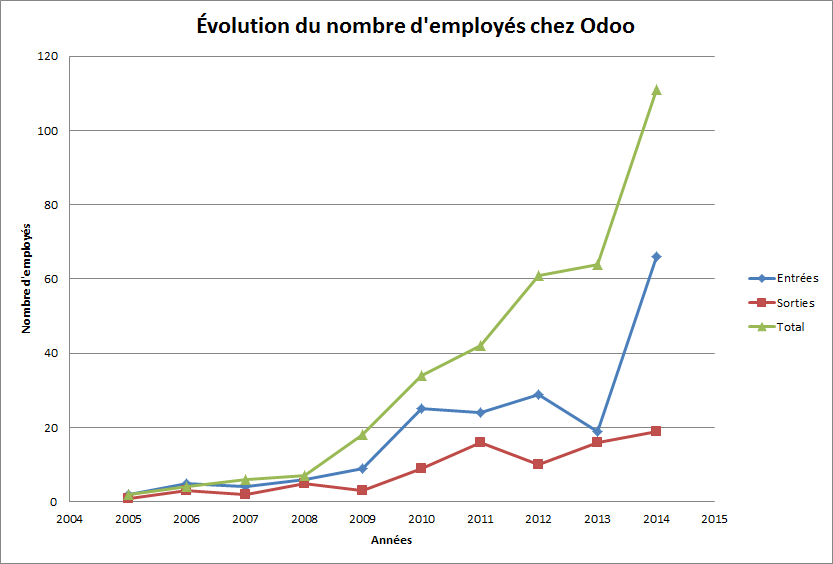
\includegraphics[scale=0.6]{document/evolution.png}
        \caption{}
        \label{}
    \end{center}
\end{figure}
\begin{table}[ht!]
    \caption{ Évolution du nombre d'employés chez Odoo en Belgique. Source: Bilan déposé à la BNB de 2005 à 2015\cite{bnb}}
    \label{nb_employe}

    \begin{center}
        \begin{tabular}{|cccc|}
             \hline
             Année & Entrées & Sortie & Total \\
             \hline
             2005 & 2  & 1  & 2   \\
             2006 & 5  & 3  & 4   \\
             2007 & 4  & 2  & 6   \\
             2008 & 7  & 5  & 7   \\
             2009 & 9  & 3  & 18  \\
             2010 & 25 & 9  & 34  \\
             2011 & 24 & 16 & 42  \\
             2012 & 29 & 10 & 61  \\
             2013 & 19 & 16 & 64  \\
             2014 & 66 & 19 & 111 \\
             \hline
        \end{tabular}
    \end{center}
\end{table}





\chapter{Odoo Appraisal Form}
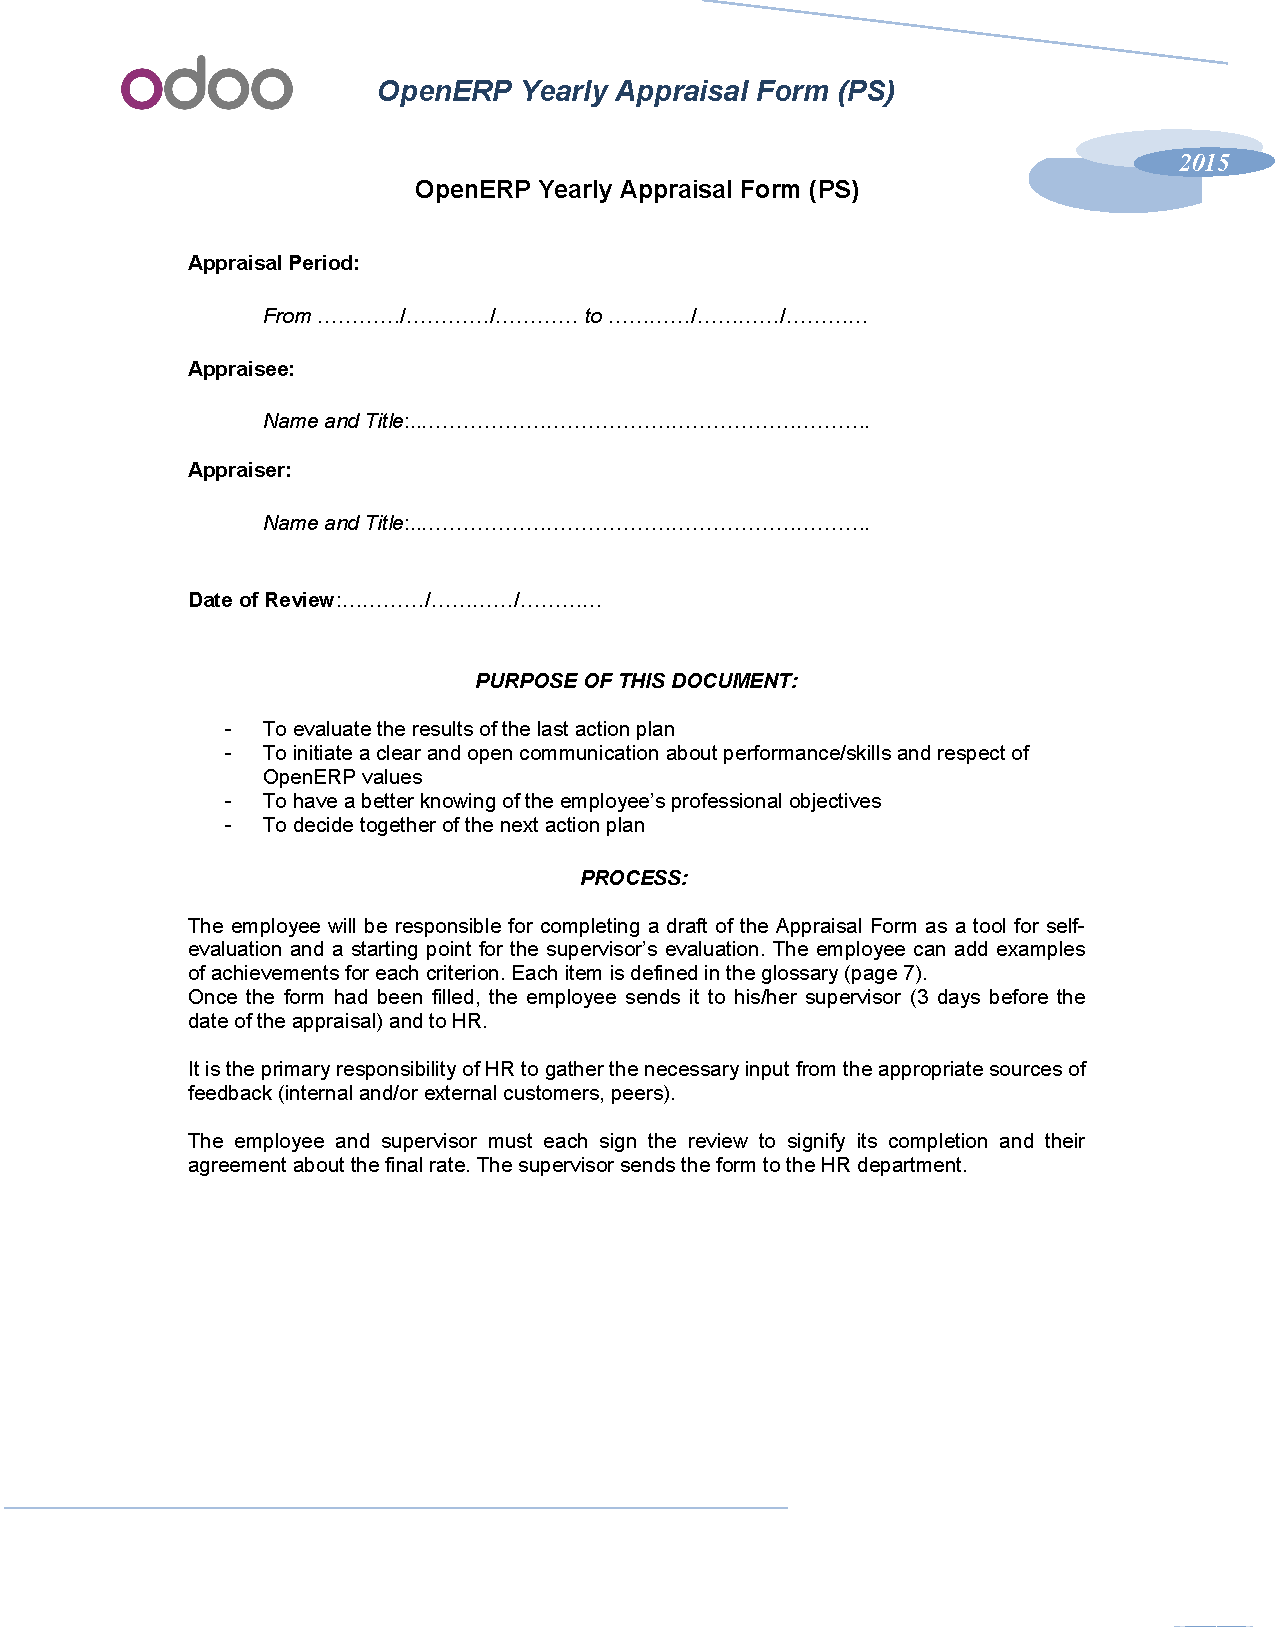
\includepdf[pages=1-6]{document/Odoo_appraisal.pdf}


\addtocontents{toc}{\vspace{2em}}  % Add a gap in the Contents, for aesthetics



\end{document}
